\documentclass{tls}

\usepackage{qtree}
\usepackage{gb4e}
% \usepackage{float}

\bibliographystyle{tlslike}

\title{Title of your TLS paper}
\author{Beatrice McHuggins and Harold Q. Snodgrass}
\institution{University of Texas at Austin}
\email{beatricemc@utexas.edu, hqs@utexas.edu}

% OT 'hand'
\usepackage{pifont}
\newcommand{\hand}{\ding{43}}

\begin{document}

\maketitle
\thispagestyle{empty}

\begin{abstract}
  This document both describes and exemplifies the TLS proceedings format. You can use the \LaTeX{} source as a template for your submission (highly recommended), or the rendered PDF as a model for how your document should end up looking. The sections below specify requirements for the paper and supply examples for how to typeset common linguistic phenomena in \LaTeX.
\end{abstract}

\section{Introduction}

The following rules apply to all submitted papers:

\begin{itemize}
  \item They must be written in English.
  \item They must contain the name(s) of the author(s).
  \item They cannot exceed 20 pages, including references, data, and appendices.
\end{itemize}

\noindent
You must submit both the final PDF as well as the original Word Document / \LaTeX{} source.

This paper template can be found on the conference website. Please use either the Microsoft Word compatible file or the \LaTeX{} format file when preparing your submission. If there are special questions or wishes regarding paper preparation and submission for TLS 15, correspondence should be addressed via email to \url{tls.conference@gmail.com}; please include ``TLS 15 Proceedings'' in the subject line of the email.


\section{Page layout and style}

The page layout should conform to the following rules. The easiest way to meet these requirements is to use the supplied templates (Word or \LaTeX) and check details against this example file. If for some reason you cannot use Word or \LaTeX, please follow these rules as carefully as possible and contact the editors at \url{tls.conference@gmail.com} for any clarifications.

\subsection{Basic layout}

Please adhere to the following basic layout parameters:

\begin{itemize}
  \item Page format should be US Letter (8.5"x11").
  \item Left and right margins are 1.5".
  \item Top and bottom margins are 1.25".
  \item The header and footer of each page should be empty; page numbers and author/title headers will be added to the document later.
  \item Check indentations and spacings by comparing with this example file.
\end{itemize}

\subsubsection{Headings}

Section headings (including sub-headings and sub-sub-headings) are left justified in boldface with the first letter capitalized and the rest of the heading in lower case. See examples in this file. No more than three levels of headings should be used.

\subsection{Font faces}

11 point Times or Times New Roman font is used for the main text. Other font types may be used if needed for special purposes. If you are using special fonts such as SIL IPA or Arboreal, please advise us which fonts you have made use of, and include them with your submission.

You can use phonetic symbols and special characters in your paper. For \LaTeX{} users, we recommend using the \texttt{tipa} package. If you are using Word, please include the font file along with the Word document in your submission. To make sure that readers of your article can see the phonetic symbols in the PDF document, all special symbols must be embedded in the PDF.

Depending on your text processor, you may need to configure it to `embed all fonts' when rendering the final PDF file.

\subsection{Figures}

All figures should be centered on the page. Figure captions should follow each
figure and have the format given in Fig.~\ref{fig:vowels}.

\begin{figure}[ht]
  \begin{center}
    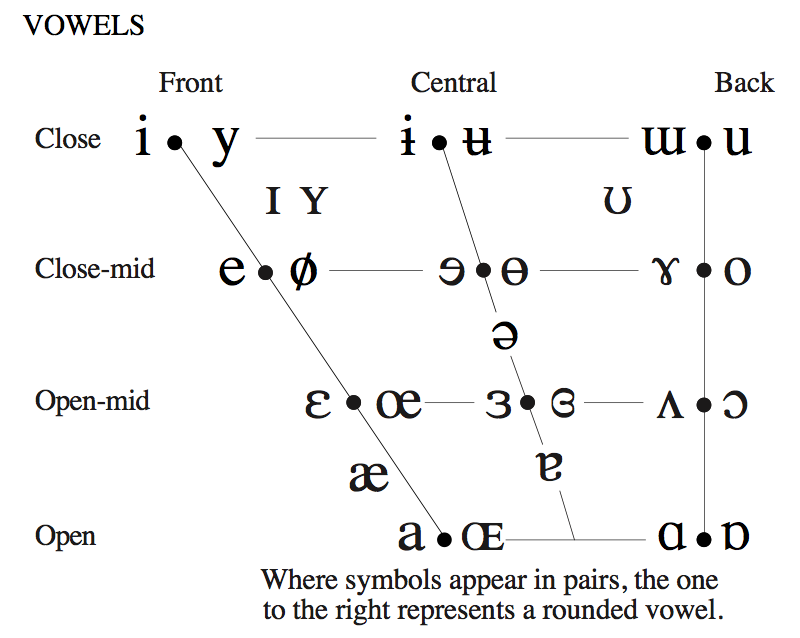
\includegraphics[width=3in]{Example-IPA.png}
  \end{center}
  \caption{The vowel chart used in the International Phonetic Alphabet (IPA).}
  \label{fig:vowels}
\end{figure}

Figures should preferably be line drawings. If they contain gray shades, it should be checked that they print well on a high-quality non-color laser printer. Color figures should not be used.

\subsection{Tables}

An example of a table is shown as Table~\ref{tab:decibel}. Somewhat different styles are allowed according to the type and purpose of the table. Color should not be used, but gray shading is allowed. There should be a margin of 6 pt above and below the table. The caption text may be above or below the table, but this should be consistent throughout the submission.

\begin{table}[ht]
  \begin{center}
    \begin{tabular}{|c|c|}
      \hline
      \rowcolor[gray]{.75}
      \hline
      ratio    & Decibels \\
      \hline
      $1/1$    & $0$   \\
      $2/1$    & $6$   \\
      $10/1$   & $20$  \\
      $100/1$  & $40$  \\
      $1000/1$ & $60$  \\
      \hline
    \end{tabular}
  \end{center}
  \caption{This is an example of a table showing Decibel (dB) ratios.}
  \label{tab:decibel}
\end{table}

\subsection{Examples}

If you are using Word, please insure that your example numbers are consistent with your text references. If you are using \LaTeX, we recommend using the \texttt{gb4e} package. It's not perfect, but it allows for sub-examples (which are not supported by the \texttt{equation} environment).

\begin{exe}
  \ex\label{ex1}
    \begin{xlist}
      \ex\label{ex1a} This is an English example.
      \ex\label{ex1b} This is a longer English example.
    \end{xlist}
  \ex\label{ex2} Here is a free-standing example.
\end{exe}

Example (\ref{ex1}) contains two sub-examples: (\ref{ex1a}) and (\ref{ex1b}).

\subsubsection{Equations}

If you are using \LaTeX, do not use the \texttt{equation} macros, as they use a different counter that does not integrate with \texttt{gb4e}'s counter. To typeset a formula in math mode, use the \$ ... \$ delimiters.

\begin{exe}
  \ex $t_0 = \frac{1}{f_0}$
\end{exe}

\subsubsection{Interlinear glosses}

How you keep your glosses lined up properly depends on the software you are using. If you are using Word, please insert your glosses inside a table, with the borders of the table set to ``none'' so that they are not visible. If you are using \LaTeX, we recommend the \texttt{$\backslash$gll} function of \texttt{gb4e.sty}.

\begin{exe}
  \ex
    \gll \textit{Los} \textit{niños} \textit{le} \textit{molestan}\\
         the-{\sc pl} children {\sc dat} bother\\
    \glt `Children irritate him.'
\end{exe}

\subsection{OT tableaux}
In Word, Optimality Theory (OT) tableaux should be implemented as standard tables.
In \LaTeX, OT tableaux should be implemented within the standard \texttt{tabular} environment. If you wish to make use of any other packages, such as \texttt{arydshln}, please include the style file when submitting your paper.

\begin{exe}
  \ex
  \begin{tabular}{|lc|c|c|c|}
    \hline
          & \textbf{input}       & {\sc Can_{1}} &  {\sc Can_{2}} & {\sc Can_{3}} \\
    \hline
    \hline
    \hand & \textit{candidate a} &    &  *                    & \cellcolor{lightgray} * \\
    \hline
          & \textit{candidate b} &    &  *!                   & \cellcolor{lightgray}   \\
    \hline
          & \textit{candidate c} & *! & \cellcolor{lightgray} & \cellcolor{lightgray}   \\
    \hline
  \end{tabular}

\end{exe}

\subsection{Syntactic trees}

Microsoft Word users should be sure to include any special fonts used to generate syntactic trees, where ``special'' is defined as ``not included as part of the standard MS Word distribution.'' For \LaTeX{} users, we recommend the \texttt{qtree} package.

\begin{exe}
  \ex
    \Tree
    [.IP
      [ Roses ].NP_i
      [.I\1 [ are ].I^0
        [.VP t_i
          [
            [ going ].V^0
            \qroof{out of style}.PP
          ].V\1
        ].VP
      ].I\1
    ]
\end{exe}

\subsection{References}

Please use LSA style: \texttt{name (year)} or \texttt{(Name year)}.  Formulations with author names like ``\ldots as \namecite{Ladefoged:2003} showed that \ldots'' are acceptable, but not ``as shown in [Ladefoged, 2003]'' or ``as shown in (Ladefoged~[6]).'' See Section 4 for more on references.

\subsection{Hyperlinks}

Links to URLs or email addresses should be formatted as normal text, not as hyperlinks (not blue or underlined, etc.). Usually hyperlinks to web pages are listed in the references section (e.g. \citeboth{Praat}). If required, line breaks can be placed within URLs after slashes or dashes, but double check that no hyphens are inserted.

\subsection{Footnotes}

This is an example of a footnote.\footnote{Remember that these are footnotes, not places to go off on multi-paragraph rants.}


\section{PDF details}

PDF files submitted must comply with the following requirements:

\begin{enumerate}
  \item All special fonts and symbols must be embedded in the PDF file so that correct rendering of the PDF does not depend on the fonts installed on the viewer's computer.
  \item There must be no password protection on the PDF file.
  \item PDF files must not be protected in any way. Content extraction, document assembly, high-resolution printing, etc., must not be forbidden.
  \item PDF files should not contain any colors, hyperlinks, multimedia or 3D content, JavaScript, or forms.
\end{enumerate}

\section{Format of references}

Monographs such as \namecite{Fant:1960} consist of author(s) last name(s), initial of the first name(s), year of publication, title in italics, location of the publication, and publisher. The names of multiple authors are separated by commas listed in the sequence last name, comma, initial(s) of the first name(s) (cf. the examples \citeboth{Beattie/etal:1982}, \citeboth{Peterson/Barney:1952}).

Contributions to volumes, e.g., \namecite{Stevens:1999}, follow the convention that the title of the volume is in italics, but not the title of the contribution. Book editors should appear after the book title, followed by page numbers, place of publication, and publisher.

Journal articles should be handled in the same way as contributions to volumes, except that the title of the journal is in italics and the editors are not listed. Longer names of well-known journals can be abbreviated (e.g., \citeboth{Peterson/Barney:1952}).

Articles in conference proceedings such as \namecite{Ladefoged:2003} are referenced in the same way as journal articles. The word ``proceedings'' can be abbreviated and the location should be mentioned after the name of the conference. Here, abbreviations of well-known conferences are possible.

\bibliography{Example}

\end{document}
